% =====================================================================
%  DORI architecture, simplified version. Cleaned-up mathcha export.
%  Standalone file: it changes nothing else in your project.
%
%  Use it with:  \resizebox{\linewidth}{!}{% =====================================================================
%  DORI architecture, simplified version. Cleaned-up mathcha export.
%  Standalone file: it changes nothing else in your project.
%
%  Use it with:  \resizebox{\linewidth}{!}{% =====================================================================
%  DORI architecture, simplified version. Cleaned-up mathcha export.
%  Standalone file: it changes nothing else in your project.
%
%  Use it with:  \resizebox{\linewidth}{!}{% =====================================================================
%  DORI architecture, simplified version. Cleaned-up mathcha export.
%  Standalone file: it changes nothing else in your project.
%
%  Use it with:  \resizebox{\linewidth}{!}{\input{architecture_simple.tex}}
%  Needs \usepackage{tikz} in the preamble. Nothing else.
%
%  WHAT WAS WRONG AND WHAT I CHANGED
%
%  0. The paste was a single line. The first mathcha comment, "%set default
%     line width", then swallows the whole picture, because a % comments out
%     the rest of its LINE. Pasted as one line it compiles to an empty page.
%     Everything below is therefore one command per line. Keep it that way.
%
%  1. Labels that mathcha had flattened into text:
%       Vbias                                  -> $V_{bias}$
%       \textbackslash (\textbackslash propto...) -> $\propto h\nu$
%       N Bin \ E                              -> $N_{\mathrm{bin}} \propto E$
%
%  2. The three block names were fixed-width minipages, so the two lines used
%     the OUTER font's baseline skip (12 pt) while the text was 5 pt. That is
%     why "Pulse" and "Shaping" were flung apart and spilled out of every
%     shape. They are now single centred nodes placed on each shape's centre,
%     at 4 pt, which is the largest size at which "Discrimination" fits inside
%     the green box. Scaled to a 22.6 cm poster column that prints at 19 pt.
%
%  3. Geometry snapped so the dimensions agree:
%       - digitalization block moved to the green block's exact top and
%         bottom (230.17 and 260.47); it was 0.7 units out
%       - the arrow between the two blocks now runs edge to edge, 57.17 to
%         64.30, on their shared centre line y = 245.32
%       - the shaping-to-discrimination arrow now leaves the triangle edge at
%         its mid height (49.21, 206.69) and lands exactly on the box top
%       - the three waveform baselines were sloping by 0.2 units each; all
%         three are now exactly horizontal, and the digitised one sits on the
%         bottom edge of its block
%
%  4. Colours were already yours, so they are untouched: 26,111,223 blue,
%     55,173,107 green, 241,74,64 red, 204,153,0 for the X-ray.
%
%  Nothing else was moved. Every other coordinate is exactly as you drew it.
% =====================================================================

\tikzset{every picture/.style={line width=0.75pt}}
%set default line width to 0.75pt 
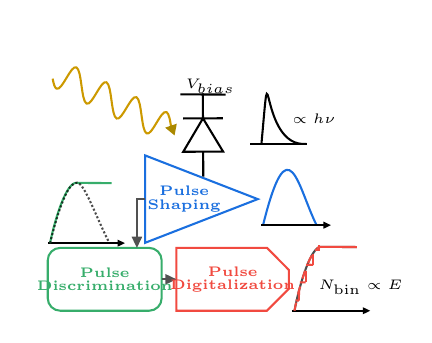
\begin{tikzpicture}[x=0.75pt,y=0.75pt,yscale=-1,xscale=1]
%uncomment if require: \path (0,623);
%set diagram left start at 0, and has height of 623
%Shape: Triangle [id:dp7568885508488827]
\draw [color={rgb, 255:red, 26; green, 111; blue, 223 } ,draw opacity=1 ][fill={rgb, 255:red, 255; green, 255; blue, 255 } ,fill opacity=1 ] (103.47,206.69) -- (49.21,227.74) -- (49.21,185.64) -- cycle ;
%Curve Lines [id:da31175352604231354]
\draw [color={rgb, 255:red, 26; green, 111; blue, 223 } ,draw opacity=1 ] (106.02,219.24) .. controls (118.37,169.32) and (122.81,201.41) .. (131.83,219.24) ;
%Straight Lines [id:da8734375505712497]
\draw (105.11,219.24) -- (135.72,219.24) ;
\draw [shift={(138.71,219.24)}, rotate = 180] [fill={rgb, 255:red, 0; green, 0; blue, 0 } ][line width=0.08] [draw opacity=0] (3.57,-1.72) -- (0,0) -- (3.57,1.72) -- cycle ;
%Straight Lines [id:da8033158731026477]
\draw (2.40,227.90) -- (36.47,227.90) ;
\draw [shift={(39.47,227.90)}, rotate = 180] [fill={rgb, 255:red, 0; green, 0; blue, 0 } ][line width=0.08] [draw opacity=0] (3.57,-1.72) -- (0,0) -- (3.57,1.72) -- cycle ;
%Curve Lines [id:da8165839321439692]
\draw [color={rgb, 255:red, 55; green, 173; blue, 107 } ,draw opacity=1 ] (3.4,227.9) .. controls (4.98,219.77) and (10.29,199.92) .. (15.62,198.87) ;
%Straight Lines [id:da9249993527350234]
\draw [color={rgb, 255:red, 55; green, 173; blue, 107 } ,draw opacity=1 ] (15.62,198.87) -- (33.07,198.97) ;
%Curve Lines [id:da01278581006202073]
\draw [color={rgb, 255:red, 0; green, 0; blue, 0 } ,draw opacity=0.7 ] [dash pattern={on 0.75pt off 0.75pt on 0.75pt off 0.75pt}] (3.4,227.9) .. controls (8.86,206.12) and (12.92,198.66) .. (16.46,198.78) .. controls (20,198.9) and (25.91,216.13) .. (31.88,227.63) ;
%Snip Same Side Corner Rect [id:dp24267720786095204]
\draw [color={rgb, 255:red, 241; green, 74; blue, 64 } ,draw opacity=1 ][fill={rgb, 255:red, 255; green, 255; blue, 255 } ,fill opacity=1 ] (107.91,230.17) -- (118.43,240.77) -- (118.43,249.87) -- (107.91,260.47) -- (64.30,260.47) -- (64.30,230.17) -- cycle ;
%Straight Lines [id:da44513384727711636]
\draw (120.16,260.47) -- (154.65,260.47) ;
\draw [shift={(157.65,260.47)}, rotate = 180] [fill={rgb, 255:red, 0; green, 0; blue, 0 } ][line width=0.08] [draw opacity=0] (3.57,-1.72) -- (0,0) -- (3.57,1.72) -- cycle ;
%Curve Lines [id:da06577028557977793]
\draw [color={rgb, 255:red, 0; green, 0; blue, 0 } ,draw opacity=0.7 ] (121.17,260.47) .. controls (122.76,251.66) and (128.14,230.78) .. (133.53,229.68) ;
%Straight Lines [id:da0572237289311508]
\draw [color={rgb, 255:red, 0; green, 0; blue, 0 } ,draw opacity=0.7 ] (133.53,229.68) -- (151.18,229.78) ;
%Curve Lines [id:da3804043288541633]
\draw [color={rgb, 255:red, 241; green, 74; blue, 64 } ,draw opacity=1 ] [dash pattern={on 3pt off 3pt on 3pt off 3pt}] (121.17,260.47) .. controls (122.76,251.66) and (128.14,230.78) .. (133.53,229.68) ;
%Straight Lines [id:da5333998307295363]
\draw [color={rgb, 255:red, 241; green, 74; blue, 64 } ,draw opacity=1 ] (121.74,255.47) -- (123.27,255.6) ;
%Straight Lines [id:da40393427405433224]
\draw [color={rgb, 255:red, 241; green, 74; blue, 64 } ,draw opacity=1 ] (123.27,255.6) -- (123.36,250.91) ;
%Straight Lines [id:da3824884565346163]
\draw [color={rgb, 255:red, 241; green, 74; blue, 64 } ,draw opacity=1 ] (131.13,231.25) -- (133.67,231.25) ;
%Straight Lines [id:da8760345808356574]
\draw [color={rgb, 255:red, 241; green, 74; blue, 64 } ,draw opacity=1 ] (133.04,231.56) -- (133.04,228.9) ;
%Straight Lines [id:da012864593156911797]
\draw [color={rgb, 255:red, 241; green, 74; blue, 64 } ,draw opacity=1 ] (123.79,246.76) -- (126.58,246.84) ;
%Straight Lines [id:da7563678124476333]
\draw [color={rgb, 255:red, 241; green, 74; blue, 64 } ,draw opacity=1 ] (126.58,246.84) -- (126.58,241.47) ;
%Straight Lines [id:da5333243365793827]
\draw [color={rgb, 255:red, 241; green, 74; blue, 64 } ,draw opacity=1 ] (127.57,238.34) -- (126.82,238.29) -- (130.11,238.35) ;
%Straight Lines [id:da6175946543817453]
\draw [color={rgb, 255:red, 241; green, 74; blue, 64 } ,draw opacity=1 ] (130.11,238.35) -- (130.11,237.66) -- (130.11,237.63) -- (130.11,232.98) ;
%Straight Lines [id:da3521344691026579]
\draw [color={rgb, 255:red, 241; green, 74; blue, 64 } ,draw opacity=1 ] (133.53,229.68) -- (151.18,229.78) ;
%Straight Lines [id:da5320121248918265]
\draw (66.17,156.23) -- (88.04,156.31) ;
%Shape: Diode [id:dp5726237104125548]
\draw (67.56,183.88) -- (77.08,167.78) -- (86.77,183.78) -- (67.56,183.88) -- cycle (77.23,195.87) -- (77.17,183.83) (67.47,167.83) -- (86.68,167.73) (77.08,167.78) -- (77.01,155.74) ;
%Curve Lines [id:da7636399085738066]
\draw [color={rgb, 255:red, 0; green, 0; blue, 0 } ,draw opacity=1 ][fill={rgb, 255:red, 255; green, 255; blue, 255 } ,fill opacity=1 ] (105.25,180.06) .. controls (110.26,124.59) and (103.64,182.32) .. (126.96,180.06) ;
%Straight Lines [id:da4842235537927333]
\draw (99.83,180.06) -- (126.96,180.06) ;
%Shape: Wave [id:dp9368433800430482]
\draw [color={rgb, 255:red, 204; green, 153; blue, 0 } ,draw opacity=1 ] (4.66,148.65) .. controls (5.1,151.11) and (5.63,153.03) .. (6.51,153.46) .. controls (7.82,154.11) and (9.52,151.3) .. (11.3,148.33) .. controls (13.08,145.37) and (14.78,142.56) .. (16.09,143.21) .. controls (17.4,143.86) and (17.96,147.8) .. (18.54,151.93) .. controls (19.12,156.06) and (19.67,160) .. (20.98,160.65) .. controls (22.29,161.3) and (23.99,158.48) .. (25.77,155.52) .. controls (27.55,152.56) and (29.25,149.75) .. (30.56,150.4) .. controls (31.87,151.05) and (32.43,154.98) .. (33,159.12) .. controls (33.58,163.25) and (34.14,167.19) .. (35.45,167.84) .. controls (36.76,168.49) and (38.46,165.67) .. (40.24,162.71) .. controls (42.02,159.75) and (43.72,156.94) .. (45.03,157.59) .. controls (46.34,158.24) and (46.89,162.17) .. (47.47,166.31) .. controls (48.05,170.44) and (48.61,174.38) .. (49.92,175.03) .. controls (51.23,175.68) and (52.93,172.86) .. (54.71,169.9) .. controls (56.49,166.94) and (58.19,164.12) .. (59.5,164.77) .. controls (60.71,165.37) and (61.27,168.78) .. (61.81,172.55) ;
%Shape: Triangle [id:dp9985044017508556]
\draw [color={rgb, 255:red, 170; green, 136; blue, 0 } ,draw opacity=1 ][fill={rgb, 255:red, 170; green, 136; blue, 0 } ,fill opacity=1 ] (63.05,175.07) -- (59.86,172.44) -- (63.81,171.09) -- cycle ;
%Rounded Rect [id:dp19934922796405263]
\draw [color={rgb, 255:red, 55; green, 173; blue, 107 } ,draw opacity=1 ] (2.28,236.23) .. controls (2.28,232.88) and (4.99,230.17) .. (8.34,230.17) -- (51.1,230.17) .. controls (54.45,230.17) and (57.17,232.88) .. (57.17,236.23) -- (57.17,254.41) .. controls (57.17,257.75) and (54.45,260.47) .. (51.1,260.47) -- (8.34,260.47) .. controls (4.99,260.47) and (2.28,257.75) .. (2.28,254.41) -- cycle ;
%Straight Lines [id:da2933898096984766]
\draw [color={rgb, 255:red, 81; green, 81; blue, 81 } ,draw opacity=1 ] (49.21,206.69) -- (45.25,206.69) -- (45.25,227.17) ;
\draw [shift={(45.25,230.17)}, rotate = 270] [fill={rgb, 255:red, 81; green, 81; blue, 81 } ,fill opacity=1 ][line width=0.08] [draw opacity=0] (5.36,-2.57) -- (0,0) -- (5.36,2.57) -- cycle ;
%Straight Lines [id:da15405365263406912]
\draw [color={rgb, 255:red, 81; green, 81; blue, 81 } ,draw opacity=1 ] (57.17,245.32) -- (61.30,245.32) ;
\draw [shift={(64.30,245.32)}, rotate = 180] [fill={rgb, 255:red, 81; green, 81; blue, 81 } ,fill opacity=1 ][line width=0.08] [draw opacity=0] (5.36,-2.57) -- (0,0) -- (5.36,2.57) -- cycle ;
% Text Node
\draw (68.00,206.69) node [anchor=center, align=center, font=\fontsize{4}{4.8}\selectfont\bfseries, color={rgb, 255:red, 26; green, 111; blue, 223 }] {Pulse\\Shaping};
% Text Node
\draw (131.29,244.42) node [anchor=north west][inner sep=0.75pt] [font=\tiny] [align=left] {$N_{\mathrm{bin}} \propto E$};
% Text Node
\draw (67.3,147.49) node [anchor=north west][inner sep=0.75pt] [font=\tiny] [align=left] {$V_{bias}$};
% Text Node
\draw (118.7,164.21) node [anchor=north west][inner sep=0.75pt] [font=\tiny] [align=left] {$\propto h\nu$};
% Text Node
\draw (29.73,245.32) node [anchor=center, align=center, font=\fontsize{4}{4.8}\selectfont\bfseries, color={rgb, 255:red, 55; green, 173; blue, 107 }] {Pulse\\Discrimination};
% Text Node
\draw (91.37,245.32) node [anchor=center, align=center, font=\fontsize{4}{4.8}\selectfont\bfseries, color={rgb, 255:red, 241; green, 74; blue, 64 }] {Pulse\\Digitalization};
\end{tikzpicture}
}
%  Needs \usepackage{tikz} in the preamble. Nothing else.
%
%  WHAT WAS WRONG AND WHAT I CHANGED
%
%  0. The paste was a single line. The first mathcha comment, "%set default
%     line width", then swallows the whole picture, because a % comments out
%     the rest of its LINE. Pasted as one line it compiles to an empty page.
%     Everything below is therefore one command per line. Keep it that way.
%
%  1. Labels that mathcha had flattened into text:
%       Vbias                                  -> $V_{bias}$
%       \textbackslash (\textbackslash propto...) -> $\propto h\nu$
%       N Bin \ E                              -> $N_{\mathrm{bin}} \propto E$
%
%  2. The three block names were fixed-width minipages, so the two lines used
%     the OUTER font's baseline skip (12 pt) while the text was 5 pt. That is
%     why "Pulse" and "Shaping" were flung apart and spilled out of every
%     shape. They are now single centred nodes placed on each shape's centre,
%     at 4 pt, which is the largest size at which "Discrimination" fits inside
%     the green box. Scaled to a 22.6 cm poster column that prints at 19 pt.
%
%  3. Geometry snapped so the dimensions agree:
%       - digitalization block moved to the green block's exact top and
%         bottom (230.17 and 260.47); it was 0.7 units out
%       - the arrow between the two blocks now runs edge to edge, 57.17 to
%         64.30, on their shared centre line y = 245.32
%       - the shaping-to-discrimination arrow now leaves the triangle edge at
%         its mid height (49.21, 206.69) and lands exactly on the box top
%       - the three waveform baselines were sloping by 0.2 units each; all
%         three are now exactly horizontal, and the digitised one sits on the
%         bottom edge of its block
%
%  4. Colours were already yours, so they are untouched: 26,111,223 blue,
%     55,173,107 green, 241,74,64 red, 204,153,0 for the X-ray.
%
%  Nothing else was moved. Every other coordinate is exactly as you drew it.
% =====================================================================

\tikzset{every picture/.style={line width=0.75pt}}
%set default line width to 0.75pt 
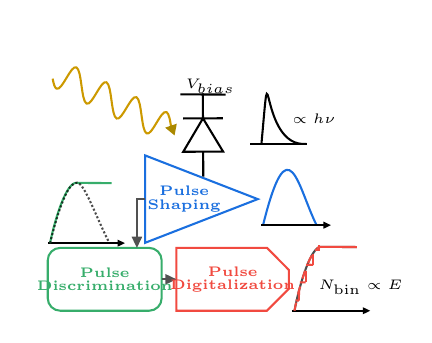
\begin{tikzpicture}[x=0.75pt,y=0.75pt,yscale=-1,xscale=1]
%uncomment if require: \path (0,623);
%set diagram left start at 0, and has height of 623
%Shape: Triangle [id:dp7568885508488827]
\draw [color={rgb, 255:red, 26; green, 111; blue, 223 } ,draw opacity=1 ][fill={rgb, 255:red, 255; green, 255; blue, 255 } ,fill opacity=1 ] (103.47,206.69) -- (49.21,227.74) -- (49.21,185.64) -- cycle ;
%Curve Lines [id:da31175352604231354]
\draw [color={rgb, 255:red, 26; green, 111; blue, 223 } ,draw opacity=1 ] (106.02,219.24) .. controls (118.37,169.32) and (122.81,201.41) .. (131.83,219.24) ;
%Straight Lines [id:da8734375505712497]
\draw (105.11,219.24) -- (135.72,219.24) ;
\draw [shift={(138.71,219.24)}, rotate = 180] [fill={rgb, 255:red, 0; green, 0; blue, 0 } ][line width=0.08] [draw opacity=0] (3.57,-1.72) -- (0,0) -- (3.57,1.72) -- cycle ;
%Straight Lines [id:da8033158731026477]
\draw (2.40,227.90) -- (36.47,227.90) ;
\draw [shift={(39.47,227.90)}, rotate = 180] [fill={rgb, 255:red, 0; green, 0; blue, 0 } ][line width=0.08] [draw opacity=0] (3.57,-1.72) -- (0,0) -- (3.57,1.72) -- cycle ;
%Curve Lines [id:da8165839321439692]
\draw [color={rgb, 255:red, 55; green, 173; blue, 107 } ,draw opacity=1 ] (3.4,227.9) .. controls (4.98,219.77) and (10.29,199.92) .. (15.62,198.87) ;
%Straight Lines [id:da9249993527350234]
\draw [color={rgb, 255:red, 55; green, 173; blue, 107 } ,draw opacity=1 ] (15.62,198.87) -- (33.07,198.97) ;
%Curve Lines [id:da01278581006202073]
\draw [color={rgb, 255:red, 0; green, 0; blue, 0 } ,draw opacity=0.7 ] [dash pattern={on 0.75pt off 0.75pt on 0.75pt off 0.75pt}] (3.4,227.9) .. controls (8.86,206.12) and (12.92,198.66) .. (16.46,198.78) .. controls (20,198.9) and (25.91,216.13) .. (31.88,227.63) ;
%Snip Same Side Corner Rect [id:dp24267720786095204]
\draw [color={rgb, 255:red, 241; green, 74; blue, 64 } ,draw opacity=1 ][fill={rgb, 255:red, 255; green, 255; blue, 255 } ,fill opacity=1 ] (107.91,230.17) -- (118.43,240.77) -- (118.43,249.87) -- (107.91,260.47) -- (64.30,260.47) -- (64.30,230.17) -- cycle ;
%Straight Lines [id:da44513384727711636]
\draw (120.16,260.47) -- (154.65,260.47) ;
\draw [shift={(157.65,260.47)}, rotate = 180] [fill={rgb, 255:red, 0; green, 0; blue, 0 } ][line width=0.08] [draw opacity=0] (3.57,-1.72) -- (0,0) -- (3.57,1.72) -- cycle ;
%Curve Lines [id:da06577028557977793]
\draw [color={rgb, 255:red, 0; green, 0; blue, 0 } ,draw opacity=0.7 ] (121.17,260.47) .. controls (122.76,251.66) and (128.14,230.78) .. (133.53,229.68) ;
%Straight Lines [id:da0572237289311508]
\draw [color={rgb, 255:red, 0; green, 0; blue, 0 } ,draw opacity=0.7 ] (133.53,229.68) -- (151.18,229.78) ;
%Curve Lines [id:da3804043288541633]
\draw [color={rgb, 255:red, 241; green, 74; blue, 64 } ,draw opacity=1 ] [dash pattern={on 3pt off 3pt on 3pt off 3pt}] (121.17,260.47) .. controls (122.76,251.66) and (128.14,230.78) .. (133.53,229.68) ;
%Straight Lines [id:da5333998307295363]
\draw [color={rgb, 255:red, 241; green, 74; blue, 64 } ,draw opacity=1 ] (121.74,255.47) -- (123.27,255.6) ;
%Straight Lines [id:da40393427405433224]
\draw [color={rgb, 255:red, 241; green, 74; blue, 64 } ,draw opacity=1 ] (123.27,255.6) -- (123.36,250.91) ;
%Straight Lines [id:da3824884565346163]
\draw [color={rgb, 255:red, 241; green, 74; blue, 64 } ,draw opacity=1 ] (131.13,231.25) -- (133.67,231.25) ;
%Straight Lines [id:da8760345808356574]
\draw [color={rgb, 255:red, 241; green, 74; blue, 64 } ,draw opacity=1 ] (133.04,231.56) -- (133.04,228.9) ;
%Straight Lines [id:da012864593156911797]
\draw [color={rgb, 255:red, 241; green, 74; blue, 64 } ,draw opacity=1 ] (123.79,246.76) -- (126.58,246.84) ;
%Straight Lines [id:da7563678124476333]
\draw [color={rgb, 255:red, 241; green, 74; blue, 64 } ,draw opacity=1 ] (126.58,246.84) -- (126.58,241.47) ;
%Straight Lines [id:da5333243365793827]
\draw [color={rgb, 255:red, 241; green, 74; blue, 64 } ,draw opacity=1 ] (127.57,238.34) -- (126.82,238.29) -- (130.11,238.35) ;
%Straight Lines [id:da6175946543817453]
\draw [color={rgb, 255:red, 241; green, 74; blue, 64 } ,draw opacity=1 ] (130.11,238.35) -- (130.11,237.66) -- (130.11,237.63) -- (130.11,232.98) ;
%Straight Lines [id:da3521344691026579]
\draw [color={rgb, 255:red, 241; green, 74; blue, 64 } ,draw opacity=1 ] (133.53,229.68) -- (151.18,229.78) ;
%Straight Lines [id:da5320121248918265]
\draw (66.17,156.23) -- (88.04,156.31) ;
%Shape: Diode [id:dp5726237104125548]
\draw (67.56,183.88) -- (77.08,167.78) -- (86.77,183.78) -- (67.56,183.88) -- cycle (77.23,195.87) -- (77.17,183.83) (67.47,167.83) -- (86.68,167.73) (77.08,167.78) -- (77.01,155.74) ;
%Curve Lines [id:da7636399085738066]
\draw [color={rgb, 255:red, 0; green, 0; blue, 0 } ,draw opacity=1 ][fill={rgb, 255:red, 255; green, 255; blue, 255 } ,fill opacity=1 ] (105.25,180.06) .. controls (110.26,124.59) and (103.64,182.32) .. (126.96,180.06) ;
%Straight Lines [id:da4842235537927333]
\draw (99.83,180.06) -- (126.96,180.06) ;
%Shape: Wave [id:dp9368433800430482]
\draw [color={rgb, 255:red, 204; green, 153; blue, 0 } ,draw opacity=1 ] (4.66,148.65) .. controls (5.1,151.11) and (5.63,153.03) .. (6.51,153.46) .. controls (7.82,154.11) and (9.52,151.3) .. (11.3,148.33) .. controls (13.08,145.37) and (14.78,142.56) .. (16.09,143.21) .. controls (17.4,143.86) and (17.96,147.8) .. (18.54,151.93) .. controls (19.12,156.06) and (19.67,160) .. (20.98,160.65) .. controls (22.29,161.3) and (23.99,158.48) .. (25.77,155.52) .. controls (27.55,152.56) and (29.25,149.75) .. (30.56,150.4) .. controls (31.87,151.05) and (32.43,154.98) .. (33,159.12) .. controls (33.58,163.25) and (34.14,167.19) .. (35.45,167.84) .. controls (36.76,168.49) and (38.46,165.67) .. (40.24,162.71) .. controls (42.02,159.75) and (43.72,156.94) .. (45.03,157.59) .. controls (46.34,158.24) and (46.89,162.17) .. (47.47,166.31) .. controls (48.05,170.44) and (48.61,174.38) .. (49.92,175.03) .. controls (51.23,175.68) and (52.93,172.86) .. (54.71,169.9) .. controls (56.49,166.94) and (58.19,164.12) .. (59.5,164.77) .. controls (60.71,165.37) and (61.27,168.78) .. (61.81,172.55) ;
%Shape: Triangle [id:dp9985044017508556]
\draw [color={rgb, 255:red, 170; green, 136; blue, 0 } ,draw opacity=1 ][fill={rgb, 255:red, 170; green, 136; blue, 0 } ,fill opacity=1 ] (63.05,175.07) -- (59.86,172.44) -- (63.81,171.09) -- cycle ;
%Rounded Rect [id:dp19934922796405263]
\draw [color={rgb, 255:red, 55; green, 173; blue, 107 } ,draw opacity=1 ] (2.28,236.23) .. controls (2.28,232.88) and (4.99,230.17) .. (8.34,230.17) -- (51.1,230.17) .. controls (54.45,230.17) and (57.17,232.88) .. (57.17,236.23) -- (57.17,254.41) .. controls (57.17,257.75) and (54.45,260.47) .. (51.1,260.47) -- (8.34,260.47) .. controls (4.99,260.47) and (2.28,257.75) .. (2.28,254.41) -- cycle ;
%Straight Lines [id:da2933898096984766]
\draw [color={rgb, 255:red, 81; green, 81; blue, 81 } ,draw opacity=1 ] (49.21,206.69) -- (45.25,206.69) -- (45.25,227.17) ;
\draw [shift={(45.25,230.17)}, rotate = 270] [fill={rgb, 255:red, 81; green, 81; blue, 81 } ,fill opacity=1 ][line width=0.08] [draw opacity=0] (5.36,-2.57) -- (0,0) -- (5.36,2.57) -- cycle ;
%Straight Lines [id:da15405365263406912]
\draw [color={rgb, 255:red, 81; green, 81; blue, 81 } ,draw opacity=1 ] (57.17,245.32) -- (61.30,245.32) ;
\draw [shift={(64.30,245.32)}, rotate = 180] [fill={rgb, 255:red, 81; green, 81; blue, 81 } ,fill opacity=1 ][line width=0.08] [draw opacity=0] (5.36,-2.57) -- (0,0) -- (5.36,2.57) -- cycle ;
% Text Node
\draw (68.00,206.69) node [anchor=center, align=center, font=\fontsize{4}{4.8}\selectfont\bfseries, color={rgb, 255:red, 26; green, 111; blue, 223 }] {Pulse\\Shaping};
% Text Node
\draw (131.29,244.42) node [anchor=north west][inner sep=0.75pt] [font=\tiny] [align=left] {$N_{\mathrm{bin}} \propto E$};
% Text Node
\draw (67.3,147.49) node [anchor=north west][inner sep=0.75pt] [font=\tiny] [align=left] {$V_{bias}$};
% Text Node
\draw (118.7,164.21) node [anchor=north west][inner sep=0.75pt] [font=\tiny] [align=left] {$\propto h\nu$};
% Text Node
\draw (29.73,245.32) node [anchor=center, align=center, font=\fontsize{4}{4.8}\selectfont\bfseries, color={rgb, 255:red, 55; green, 173; blue, 107 }] {Pulse\\Discrimination};
% Text Node
\draw (91.37,245.32) node [anchor=center, align=center, font=\fontsize{4}{4.8}\selectfont\bfseries, color={rgb, 255:red, 241; green, 74; blue, 64 }] {Pulse\\Digitalization};
\end{tikzpicture}
}
%  Needs \usepackage{tikz} in the preamble. Nothing else.
%
%  WHAT WAS WRONG AND WHAT I CHANGED
%
%  0. The paste was a single line. The first mathcha comment, "%set default
%     line width", then swallows the whole picture, because a % comments out
%     the rest of its LINE. Pasted as one line it compiles to an empty page.
%     Everything below is therefore one command per line. Keep it that way.
%
%  1. Labels that mathcha had flattened into text:
%       Vbias                                  -> $V_{bias}$
%       \textbackslash (\textbackslash propto...) -> $\propto h\nu$
%       N Bin \ E                              -> $N_{\mathrm{bin}} \propto E$
%
%  2. The three block names were fixed-width minipages, so the two lines used
%     the OUTER font's baseline skip (12 pt) while the text was 5 pt. That is
%     why "Pulse" and "Shaping" were flung apart and spilled out of every
%     shape. They are now single centred nodes placed on each shape's centre,
%     at 4 pt, which is the largest size at which "Discrimination" fits inside
%     the green box. Scaled to a 22.6 cm poster column that prints at 19 pt.
%
%  3. Geometry snapped so the dimensions agree:
%       - digitalization block moved to the green block's exact top and
%         bottom (230.17 and 260.47); it was 0.7 units out
%       - the arrow between the two blocks now runs edge to edge, 57.17 to
%         64.30, on their shared centre line y = 245.32
%       - the shaping-to-discrimination arrow now leaves the triangle edge at
%         its mid height (49.21, 206.69) and lands exactly on the box top
%       - the three waveform baselines were sloping by 0.2 units each; all
%         three are now exactly horizontal, and the digitised one sits on the
%         bottom edge of its block
%
%  4. Colours were already yours, so they are untouched: 26,111,223 blue,
%     55,173,107 green, 241,74,64 red, 204,153,0 for the X-ray.
%
%  Nothing else was moved. Every other coordinate is exactly as you drew it.
% =====================================================================

\tikzset{every picture/.style={line width=0.75pt}}
%set default line width to 0.75pt 
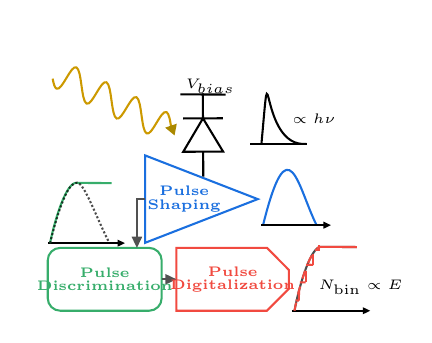
\begin{tikzpicture}[x=0.75pt,y=0.75pt,yscale=-1,xscale=1]
%uncomment if require: \path (0,623);
%set diagram left start at 0, and has height of 623
%Shape: Triangle [id:dp7568885508488827]
\draw [color={rgb, 255:red, 26; green, 111; blue, 223 } ,draw opacity=1 ][fill={rgb, 255:red, 255; green, 255; blue, 255 } ,fill opacity=1 ] (103.47,206.69) -- (49.21,227.74) -- (49.21,185.64) -- cycle ;
%Curve Lines [id:da31175352604231354]
\draw [color={rgb, 255:red, 26; green, 111; blue, 223 } ,draw opacity=1 ] (106.02,219.24) .. controls (118.37,169.32) and (122.81,201.41) .. (131.83,219.24) ;
%Straight Lines [id:da8734375505712497]
\draw (105.11,219.24) -- (135.72,219.24) ;
\draw [shift={(138.71,219.24)}, rotate = 180] [fill={rgb, 255:red, 0; green, 0; blue, 0 } ][line width=0.08] [draw opacity=0] (3.57,-1.72) -- (0,0) -- (3.57,1.72) -- cycle ;
%Straight Lines [id:da8033158731026477]
\draw (2.40,227.90) -- (36.47,227.90) ;
\draw [shift={(39.47,227.90)}, rotate = 180] [fill={rgb, 255:red, 0; green, 0; blue, 0 } ][line width=0.08] [draw opacity=0] (3.57,-1.72) -- (0,0) -- (3.57,1.72) -- cycle ;
%Curve Lines [id:da8165839321439692]
\draw [color={rgb, 255:red, 55; green, 173; blue, 107 } ,draw opacity=1 ] (3.4,227.9) .. controls (4.98,219.77) and (10.29,199.92) .. (15.62,198.87) ;
%Straight Lines [id:da9249993527350234]
\draw [color={rgb, 255:red, 55; green, 173; blue, 107 } ,draw opacity=1 ] (15.62,198.87) -- (33.07,198.97) ;
%Curve Lines [id:da01278581006202073]
\draw [color={rgb, 255:red, 0; green, 0; blue, 0 } ,draw opacity=0.7 ] [dash pattern={on 0.75pt off 0.75pt on 0.75pt off 0.75pt}] (3.4,227.9) .. controls (8.86,206.12) and (12.92,198.66) .. (16.46,198.78) .. controls (20,198.9) and (25.91,216.13) .. (31.88,227.63) ;
%Snip Same Side Corner Rect [id:dp24267720786095204]
\draw [color={rgb, 255:red, 241; green, 74; blue, 64 } ,draw opacity=1 ][fill={rgb, 255:red, 255; green, 255; blue, 255 } ,fill opacity=1 ] (107.91,230.17) -- (118.43,240.77) -- (118.43,249.87) -- (107.91,260.47) -- (64.30,260.47) -- (64.30,230.17) -- cycle ;
%Straight Lines [id:da44513384727711636]
\draw (120.16,260.47) -- (154.65,260.47) ;
\draw [shift={(157.65,260.47)}, rotate = 180] [fill={rgb, 255:red, 0; green, 0; blue, 0 } ][line width=0.08] [draw opacity=0] (3.57,-1.72) -- (0,0) -- (3.57,1.72) -- cycle ;
%Curve Lines [id:da06577028557977793]
\draw [color={rgb, 255:red, 0; green, 0; blue, 0 } ,draw opacity=0.7 ] (121.17,260.47) .. controls (122.76,251.66) and (128.14,230.78) .. (133.53,229.68) ;
%Straight Lines [id:da0572237289311508]
\draw [color={rgb, 255:red, 0; green, 0; blue, 0 } ,draw opacity=0.7 ] (133.53,229.68) -- (151.18,229.78) ;
%Curve Lines [id:da3804043288541633]
\draw [color={rgb, 255:red, 241; green, 74; blue, 64 } ,draw opacity=1 ] [dash pattern={on 3pt off 3pt on 3pt off 3pt}] (121.17,260.47) .. controls (122.76,251.66) and (128.14,230.78) .. (133.53,229.68) ;
%Straight Lines [id:da5333998307295363]
\draw [color={rgb, 255:red, 241; green, 74; blue, 64 } ,draw opacity=1 ] (121.74,255.47) -- (123.27,255.6) ;
%Straight Lines [id:da40393427405433224]
\draw [color={rgb, 255:red, 241; green, 74; blue, 64 } ,draw opacity=1 ] (123.27,255.6) -- (123.36,250.91) ;
%Straight Lines [id:da3824884565346163]
\draw [color={rgb, 255:red, 241; green, 74; blue, 64 } ,draw opacity=1 ] (131.13,231.25) -- (133.67,231.25) ;
%Straight Lines [id:da8760345808356574]
\draw [color={rgb, 255:red, 241; green, 74; blue, 64 } ,draw opacity=1 ] (133.04,231.56) -- (133.04,228.9) ;
%Straight Lines [id:da012864593156911797]
\draw [color={rgb, 255:red, 241; green, 74; blue, 64 } ,draw opacity=1 ] (123.79,246.76) -- (126.58,246.84) ;
%Straight Lines [id:da7563678124476333]
\draw [color={rgb, 255:red, 241; green, 74; blue, 64 } ,draw opacity=1 ] (126.58,246.84) -- (126.58,241.47) ;
%Straight Lines [id:da5333243365793827]
\draw [color={rgb, 255:red, 241; green, 74; blue, 64 } ,draw opacity=1 ] (127.57,238.34) -- (126.82,238.29) -- (130.11,238.35) ;
%Straight Lines [id:da6175946543817453]
\draw [color={rgb, 255:red, 241; green, 74; blue, 64 } ,draw opacity=1 ] (130.11,238.35) -- (130.11,237.66) -- (130.11,237.63) -- (130.11,232.98) ;
%Straight Lines [id:da3521344691026579]
\draw [color={rgb, 255:red, 241; green, 74; blue, 64 } ,draw opacity=1 ] (133.53,229.68) -- (151.18,229.78) ;
%Straight Lines [id:da5320121248918265]
\draw (66.17,156.23) -- (88.04,156.31) ;
%Shape: Diode [id:dp5726237104125548]
\draw (67.56,183.88) -- (77.08,167.78) -- (86.77,183.78) -- (67.56,183.88) -- cycle (77.23,195.87) -- (77.17,183.83) (67.47,167.83) -- (86.68,167.73) (77.08,167.78) -- (77.01,155.74) ;
%Curve Lines [id:da7636399085738066]
\draw [color={rgb, 255:red, 0; green, 0; blue, 0 } ,draw opacity=1 ][fill={rgb, 255:red, 255; green, 255; blue, 255 } ,fill opacity=1 ] (105.25,180.06) .. controls (110.26,124.59) and (103.64,182.32) .. (126.96,180.06) ;
%Straight Lines [id:da4842235537927333]
\draw (99.83,180.06) -- (126.96,180.06) ;
%Shape: Wave [id:dp9368433800430482]
\draw [color={rgb, 255:red, 204; green, 153; blue, 0 } ,draw opacity=1 ] (4.66,148.65) .. controls (5.1,151.11) and (5.63,153.03) .. (6.51,153.46) .. controls (7.82,154.11) and (9.52,151.3) .. (11.3,148.33) .. controls (13.08,145.37) and (14.78,142.56) .. (16.09,143.21) .. controls (17.4,143.86) and (17.96,147.8) .. (18.54,151.93) .. controls (19.12,156.06) and (19.67,160) .. (20.98,160.65) .. controls (22.29,161.3) and (23.99,158.48) .. (25.77,155.52) .. controls (27.55,152.56) and (29.25,149.75) .. (30.56,150.4) .. controls (31.87,151.05) and (32.43,154.98) .. (33,159.12) .. controls (33.58,163.25) and (34.14,167.19) .. (35.45,167.84) .. controls (36.76,168.49) and (38.46,165.67) .. (40.24,162.71) .. controls (42.02,159.75) and (43.72,156.94) .. (45.03,157.59) .. controls (46.34,158.24) and (46.89,162.17) .. (47.47,166.31) .. controls (48.05,170.44) and (48.61,174.38) .. (49.92,175.03) .. controls (51.23,175.68) and (52.93,172.86) .. (54.71,169.9) .. controls (56.49,166.94) and (58.19,164.12) .. (59.5,164.77) .. controls (60.71,165.37) and (61.27,168.78) .. (61.81,172.55) ;
%Shape: Triangle [id:dp9985044017508556]
\draw [color={rgb, 255:red, 170; green, 136; blue, 0 } ,draw opacity=1 ][fill={rgb, 255:red, 170; green, 136; blue, 0 } ,fill opacity=1 ] (63.05,175.07) -- (59.86,172.44) -- (63.81,171.09) -- cycle ;
%Rounded Rect [id:dp19934922796405263]
\draw [color={rgb, 255:red, 55; green, 173; blue, 107 } ,draw opacity=1 ] (2.28,236.23) .. controls (2.28,232.88) and (4.99,230.17) .. (8.34,230.17) -- (51.1,230.17) .. controls (54.45,230.17) and (57.17,232.88) .. (57.17,236.23) -- (57.17,254.41) .. controls (57.17,257.75) and (54.45,260.47) .. (51.1,260.47) -- (8.34,260.47) .. controls (4.99,260.47) and (2.28,257.75) .. (2.28,254.41) -- cycle ;
%Straight Lines [id:da2933898096984766]
\draw [color={rgb, 255:red, 81; green, 81; blue, 81 } ,draw opacity=1 ] (49.21,206.69) -- (45.25,206.69) -- (45.25,227.17) ;
\draw [shift={(45.25,230.17)}, rotate = 270] [fill={rgb, 255:red, 81; green, 81; blue, 81 } ,fill opacity=1 ][line width=0.08] [draw opacity=0] (5.36,-2.57) -- (0,0) -- (5.36,2.57) -- cycle ;
%Straight Lines [id:da15405365263406912]
\draw [color={rgb, 255:red, 81; green, 81; blue, 81 } ,draw opacity=1 ] (57.17,245.32) -- (61.30,245.32) ;
\draw [shift={(64.30,245.32)}, rotate = 180] [fill={rgb, 255:red, 81; green, 81; blue, 81 } ,fill opacity=1 ][line width=0.08] [draw opacity=0] (5.36,-2.57) -- (0,0) -- (5.36,2.57) -- cycle ;
% Text Node
\draw (68.00,206.69) node [anchor=center, align=center, font=\fontsize{4}{4.8}\selectfont\bfseries, color={rgb, 255:red, 26; green, 111; blue, 223 }] {Pulse\\Shaping};
% Text Node
\draw (131.29,244.42) node [anchor=north west][inner sep=0.75pt] [font=\tiny] [align=left] {$N_{\mathrm{bin}} \propto E$};
% Text Node
\draw (67.3,147.49) node [anchor=north west][inner sep=0.75pt] [font=\tiny] [align=left] {$V_{bias}$};
% Text Node
\draw (118.7,164.21) node [anchor=north west][inner sep=0.75pt] [font=\tiny] [align=left] {$\propto h\nu$};
% Text Node
\draw (29.73,245.32) node [anchor=center, align=center, font=\fontsize{4}{4.8}\selectfont\bfseries, color={rgb, 255:red, 55; green, 173; blue, 107 }] {Pulse\\Discrimination};
% Text Node
\draw (91.37,245.32) node [anchor=center, align=center, font=\fontsize{4}{4.8}\selectfont\bfseries, color={rgb, 255:red, 241; green, 74; blue, 64 }] {Pulse\\Digitalization};
\end{tikzpicture}
}
%  Needs \usepackage{tikz} in the preamble. Nothing else.
%
%  WHAT WAS WRONG AND WHAT I CHANGED
%
%  0. The paste was a single line. The first mathcha comment, "%set default
%     line width", then swallows the whole picture, because a % comments out
%     the rest of its LINE. Pasted as one line it compiles to an empty page.
%     Everything below is therefore one command per line. Keep it that way.
%
%  1. Labels that mathcha had flattened into text:
%       Vbias                                  -> $V_{bias}$
%       \textbackslash (\textbackslash propto...) -> $\propto h\nu$
%       N Bin \ E                              -> $N_{\mathrm{bin}} \propto E$
%
%  2. The three block names were fixed-width minipages, so the two lines used
%     the OUTER font's baseline skip (12 pt) while the text was 5 pt. That is
%     why "Pulse" and "Shaping" were flung apart and spilled out of every
%     shape. They are now single centred nodes placed on each shape's centre,
%     at 4 pt, which is the largest size at which "Discrimination" fits inside
%     the green box. Scaled to a 22.6 cm poster column that prints at 19 pt.
%
%  3. Geometry snapped so the dimensions agree:
%       - digitalization block moved to the green block's exact top and
%         bottom (230.17 and 260.47); it was 0.7 units out
%       - the arrow between the two blocks now runs edge to edge, 57.17 to
%         64.30, on their shared centre line y = 245.32
%       - the shaping-to-discrimination arrow now leaves the triangle edge at
%         its mid height (49.21, 206.69) and lands exactly on the box top
%       - the three waveform baselines were sloping by 0.2 units each; all
%         three are now exactly horizontal, and the digitised one sits on the
%         bottom edge of its block
%
%  4. Colours were already yours, so they are untouched: 26,111,223 blue,
%     55,173,107 green, 241,74,64 red, 204,153,0 for the X-ray.
%
%  Nothing else was moved. Every other coordinate is exactly as you drew it.
% =====================================================================

\tikzset{every picture/.style={line width=0.75pt}}
%set default line width to 0.75pt 
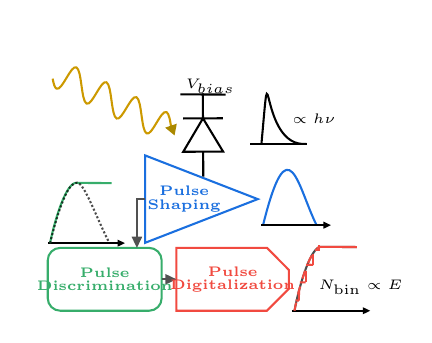
\begin{tikzpicture}[x=0.75pt,y=0.75pt,yscale=-1,xscale=1]
%uncomment if require: \path (0,623);
%set diagram left start at 0, and has height of 623
%Shape: Triangle [id:dp7568885508488827]
\draw [color={rgb, 255:red, 26; green, 111; blue, 223 } ,draw opacity=1 ][fill={rgb, 255:red, 255; green, 255; blue, 255 } ,fill opacity=1 ] (103.47,206.69) -- (49.21,227.74) -- (49.21,185.64) -- cycle ;
%Curve Lines [id:da31175352604231354]
\draw [color={rgb, 255:red, 26; green, 111; blue, 223 } ,draw opacity=1 ] (106.02,219.24) .. controls (118.37,169.32) and (122.81,201.41) .. (131.83,219.24) ;
%Straight Lines [id:da8734375505712497]
\draw (105.11,219.24) -- (135.72,219.24) ;
\draw [shift={(138.71,219.24)}, rotate = 180] [fill={rgb, 255:red, 0; green, 0; blue, 0 } ][line width=0.08] [draw opacity=0] (3.57,-1.72) -- (0,0) -- (3.57,1.72) -- cycle ;
%Straight Lines [id:da8033158731026477]
\draw (2.40,227.90) -- (36.47,227.90) ;
\draw [shift={(39.47,227.90)}, rotate = 180] [fill={rgb, 255:red, 0; green, 0; blue, 0 } ][line width=0.08] [draw opacity=0] (3.57,-1.72) -- (0,0) -- (3.57,1.72) -- cycle ;
%Curve Lines [id:da8165839321439692]
\draw [color={rgb, 255:red, 55; green, 173; blue, 107 } ,draw opacity=1 ] (3.4,227.9) .. controls (4.98,219.77) and (10.29,199.92) .. (15.62,198.87) ;
%Straight Lines [id:da9249993527350234]
\draw [color={rgb, 255:red, 55; green, 173; blue, 107 } ,draw opacity=1 ] (15.62,198.87) -- (33.07,198.97) ;
%Curve Lines [id:da01278581006202073]
\draw [color={rgb, 255:red, 0; green, 0; blue, 0 } ,draw opacity=0.7 ] [dash pattern={on 0.75pt off 0.75pt on 0.75pt off 0.75pt}] (3.4,227.9) .. controls (8.86,206.12) and (12.92,198.66) .. (16.46,198.78) .. controls (20,198.9) and (25.91,216.13) .. (31.88,227.63) ;
%Snip Same Side Corner Rect [id:dp24267720786095204]
\draw [color={rgb, 255:red, 241; green, 74; blue, 64 } ,draw opacity=1 ][fill={rgb, 255:red, 255; green, 255; blue, 255 } ,fill opacity=1 ] (107.91,230.17) -- (118.43,240.77) -- (118.43,249.87) -- (107.91,260.47) -- (64.30,260.47) -- (64.30,230.17) -- cycle ;
%Straight Lines [id:da44513384727711636]
\draw (120.16,260.47) -- (154.65,260.47) ;
\draw [shift={(157.65,260.47)}, rotate = 180] [fill={rgb, 255:red, 0; green, 0; blue, 0 } ][line width=0.08] [draw opacity=0] (3.57,-1.72) -- (0,0) -- (3.57,1.72) -- cycle ;
%Curve Lines [id:da06577028557977793]
\draw [color={rgb, 255:red, 0; green, 0; blue, 0 } ,draw opacity=0.7 ] (121.17,260.47) .. controls (122.76,251.66) and (128.14,230.78) .. (133.53,229.68) ;
%Straight Lines [id:da0572237289311508]
\draw [color={rgb, 255:red, 0; green, 0; blue, 0 } ,draw opacity=0.7 ] (133.53,229.68) -- (151.18,229.78) ;
%Curve Lines [id:da3804043288541633]
\draw [color={rgb, 255:red, 241; green, 74; blue, 64 } ,draw opacity=1 ] [dash pattern={on 3pt off 3pt on 3pt off 3pt}] (121.17,260.47) .. controls (122.76,251.66) and (128.14,230.78) .. (133.53,229.68) ;
%Straight Lines [id:da5333998307295363]
\draw [color={rgb, 255:red, 241; green, 74; blue, 64 } ,draw opacity=1 ] (121.74,255.47) -- (123.27,255.6) ;
%Straight Lines [id:da40393427405433224]
\draw [color={rgb, 255:red, 241; green, 74; blue, 64 } ,draw opacity=1 ] (123.27,255.6) -- (123.36,250.91) ;
%Straight Lines [id:da3824884565346163]
\draw [color={rgb, 255:red, 241; green, 74; blue, 64 } ,draw opacity=1 ] (131.13,231.25) -- (133.67,231.25) ;
%Straight Lines [id:da8760345808356574]
\draw [color={rgb, 255:red, 241; green, 74; blue, 64 } ,draw opacity=1 ] (133.04,231.56) -- (133.04,228.9) ;
%Straight Lines [id:da012864593156911797]
\draw [color={rgb, 255:red, 241; green, 74; blue, 64 } ,draw opacity=1 ] (123.79,246.76) -- (126.58,246.84) ;
%Straight Lines [id:da7563678124476333]
\draw [color={rgb, 255:red, 241; green, 74; blue, 64 } ,draw opacity=1 ] (126.58,246.84) -- (126.58,241.47) ;
%Straight Lines [id:da5333243365793827]
\draw [color={rgb, 255:red, 241; green, 74; blue, 64 } ,draw opacity=1 ] (127.57,238.34) -- (126.82,238.29) -- (130.11,238.35) ;
%Straight Lines [id:da6175946543817453]
\draw [color={rgb, 255:red, 241; green, 74; blue, 64 } ,draw opacity=1 ] (130.11,238.35) -- (130.11,237.66) -- (130.11,237.63) -- (130.11,232.98) ;
%Straight Lines [id:da3521344691026579]
\draw [color={rgb, 255:red, 241; green, 74; blue, 64 } ,draw opacity=1 ] (133.53,229.68) -- (151.18,229.78) ;
%Straight Lines [id:da5320121248918265]
\draw (66.17,156.23) -- (88.04,156.31) ;
%Shape: Diode [id:dp5726237104125548]
\draw (67.56,183.88) -- (77.08,167.78) -- (86.77,183.78) -- (67.56,183.88) -- cycle (77.23,195.87) -- (77.17,183.83) (67.47,167.83) -- (86.68,167.73) (77.08,167.78) -- (77.01,155.74) ;
%Curve Lines [id:da7636399085738066]
\draw [color={rgb, 255:red, 0; green, 0; blue, 0 } ,draw opacity=1 ][fill={rgb, 255:red, 255; green, 255; blue, 255 } ,fill opacity=1 ] (105.25,180.06) .. controls (110.26,124.59) and (103.64,182.32) .. (126.96,180.06) ;
%Straight Lines [id:da4842235537927333]
\draw (99.83,180.06) -- (126.96,180.06) ;
%Shape: Wave [id:dp9368433800430482]
\draw [color={rgb, 255:red, 204; green, 153; blue, 0 } ,draw opacity=1 ] (4.66,148.65) .. controls (5.1,151.11) and (5.63,153.03) .. (6.51,153.46) .. controls (7.82,154.11) and (9.52,151.3) .. (11.3,148.33) .. controls (13.08,145.37) and (14.78,142.56) .. (16.09,143.21) .. controls (17.4,143.86) and (17.96,147.8) .. (18.54,151.93) .. controls (19.12,156.06) and (19.67,160) .. (20.98,160.65) .. controls (22.29,161.3) and (23.99,158.48) .. (25.77,155.52) .. controls (27.55,152.56) and (29.25,149.75) .. (30.56,150.4) .. controls (31.87,151.05) and (32.43,154.98) .. (33,159.12) .. controls (33.58,163.25) and (34.14,167.19) .. (35.45,167.84) .. controls (36.76,168.49) and (38.46,165.67) .. (40.24,162.71) .. controls (42.02,159.75) and (43.72,156.94) .. (45.03,157.59) .. controls (46.34,158.24) and (46.89,162.17) .. (47.47,166.31) .. controls (48.05,170.44) and (48.61,174.38) .. (49.92,175.03) .. controls (51.23,175.68) and (52.93,172.86) .. (54.71,169.9) .. controls (56.49,166.94) and (58.19,164.12) .. (59.5,164.77) .. controls (60.71,165.37) and (61.27,168.78) .. (61.81,172.55) ;
%Shape: Triangle [id:dp9985044017508556]
\draw [color={rgb, 255:red, 170; green, 136; blue, 0 } ,draw opacity=1 ][fill={rgb, 255:red, 170; green, 136; blue, 0 } ,fill opacity=1 ] (63.05,175.07) -- (59.86,172.44) -- (63.81,171.09) -- cycle ;
%Rounded Rect [id:dp19934922796405263]
\draw [color={rgb, 255:red, 55; green, 173; blue, 107 } ,draw opacity=1 ] (2.28,236.23) .. controls (2.28,232.88) and (4.99,230.17) .. (8.34,230.17) -- (51.1,230.17) .. controls (54.45,230.17) and (57.17,232.88) .. (57.17,236.23) -- (57.17,254.41) .. controls (57.17,257.75) and (54.45,260.47) .. (51.1,260.47) -- (8.34,260.47) .. controls (4.99,260.47) and (2.28,257.75) .. (2.28,254.41) -- cycle ;
%Straight Lines [id:da2933898096984766]
\draw [color={rgb, 255:red, 81; green, 81; blue, 81 } ,draw opacity=1 ] (49.21,206.69) -- (45.25,206.69) -- (45.25,227.17) ;
\draw [shift={(45.25,230.17)}, rotate = 270] [fill={rgb, 255:red, 81; green, 81; blue, 81 } ,fill opacity=1 ][line width=0.08] [draw opacity=0] (5.36,-2.57) -- (0,0) -- (5.36,2.57) -- cycle ;
%Straight Lines [id:da15405365263406912]
\draw [color={rgb, 255:red, 81; green, 81; blue, 81 } ,draw opacity=1 ] (57.17,245.32) -- (61.30,245.32) ;
\draw [shift={(64.30,245.32)}, rotate = 180] [fill={rgb, 255:red, 81; green, 81; blue, 81 } ,fill opacity=1 ][line width=0.08] [draw opacity=0] (5.36,-2.57) -- (0,0) -- (5.36,2.57) -- cycle ;
% Text Node
\draw (68.00,206.69) node [anchor=center, align=center, font=\fontsize{4}{4.8}\selectfont\bfseries, color={rgb, 255:red, 26; green, 111; blue, 223 }] {Pulse\\Shaping};
% Text Node
\draw (131.29,244.42) node [anchor=north west][inner sep=0.75pt] [font=\tiny] [align=left] {$N_{\mathrm{bin}} \propto E$};
% Text Node
\draw (67.3,147.49) node [anchor=north west][inner sep=0.75pt] [font=\tiny] [align=left] {$V_{bias}$};
% Text Node
\draw (118.7,164.21) node [anchor=north west][inner sep=0.75pt] [font=\tiny] [align=left] {$\propto h\nu$};
% Text Node
\draw (29.73,245.32) node [anchor=center, align=center, font=\fontsize{4}{4.8}\selectfont\bfseries, color={rgb, 255:red, 55; green, 173; blue, 107 }] {Pulse\\Discrimination};
% Text Node
\draw (91.37,245.32) node [anchor=center, align=center, font=\fontsize{4}{4.8}\selectfont\bfseries, color={rgb, 255:red, 241; green, 74; blue, 64 }] {Pulse\\Digitalization};
\end{tikzpicture}
